\chapter{Preliminaries}

To start, we need to establish terminology and preliminary knowledge. Throughout this thesis, we will be discussing robotic arms; in robotic terms, they are more commonly referred to as \textit{manipulators}.

\begin{wrapfigure}{r}{0.25\textwidth}
    \centering
    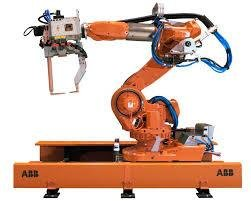
\includegraphics[width=0.35\textwidth]{Industrial-robotic-arm.jpeg}
  \caption{Industrial robotic arm with a gripper at the end\cite{manipulator}}
\end{wrapfigure}


Robotic manipulators are programmable mechanical devices, typically fixed in place. They are responsible for moving objects or tools and performing various tasks. They are widely used in factories for mass production of vehicles, electronics, etc. Based on the equipment of the specific manipulator, it can move objects from one assembly line to another, cut things, or solder parts together. However, such manipulators are often tailored to perform one specific motion repeatedly, thus, they will not be the focus of this work.

Manipulators consist of solid bodies, linked via movable joints. They often resemble human arms, although the specific shapes vary wildly.

We consider 2 basic types of joints, see Figure~\ref{fig:basicjoints}:
\begin{itemize}
  \item Revolute\footnote{Also referred to as rotary or rotational.} joints: the most common type. They consist of a motor rotating the next body around an axis. Depending on the type of motors and the build of the robot, the rotation may either be unbounded, or have a specific range of motion.
  \item Prismatic joints: these perform linear motion along the joint axis.
\end{itemize}

\begin{figure}[h]
\centering
\begin{subfigure}{.5\textwidth}
  \centering
  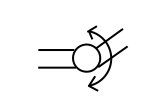
\includegraphics[width=.4\linewidth]{revolute.jpg}
  \caption{Revolute joints perform a rotation along their axis}
\end{subfigure}%
\begin{subfigure}{.5\textwidth}
  \centering
  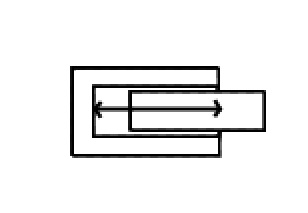
\includegraphics[width=.4\linewidth]{prismatic.png}
  \caption{Prismatic joints perform a linear motion along their axis}
\end{subfigure}
\caption{Basic joint types; the arrow refers to the respective range of motion.}
\label{fig:basicjoints}
\end{figure}

There are joint types that can perform more complicated motion, but they can generally be modelled as a combination of the basic two. Ball joints allow rotation in any direction; in a kinematic system, they can be modelled as two revolute joints in the same place. Cylindrical joints allow for both rotation and extension, serving as a combination of revolute and prismatic joints.

The state of the robot is called its configuration. A configuration is uniquely defined by two things:
\begin{itemize}
  \item The build of the robot: shape of the bodies, how they are connected, and the types of joints.
  \item The parameters of its joints.
\end{itemize}

The number of parameters that define a robotic system is referred to as degrees of freedom (DoF). Revolute and prismatic joints each have one degree of freedom. The parameter of a revolute joint is the current angle of rotation; for a prismatic joint, it's the current length it's extended at. Ball and cylindrical joints each have two degrees of freedom. The DoF of a robotic manipulator is the sum of DoFs of its flexible joints.

The end of a robotic arm is called the end effector. Typically, the end effector is different from the rest of the manipulator; it consists of a tool specialized to the robot's task. The end effector is designed to interact with the robot's environment, and there are many variatons. If the manipulator is designed to move objects, the end effector can be a fingerlike gripper, claw, or even use electromagnetic forces\cite{grippers}. In handling textile materials, the end effector can be equipped with scissors, pins or needles.

When we refer to the position of the end effector, we mean its location and rotation in cartesian space. The parameter of a joint, such as its current rotation or extension, is sometimes called its position as well; not to be confused with its position in space. Though we will see that generally, knowing the joint parameters will let us compute their position in space, and vice versa.

\section{Kinematics of robotic manipulators}

The science that studies the relationship between joint parameters and the positions in cartesian space -- particularly the end effector -- is called kinematics.
We differentiate between forward and inverse kinematics.

Forward kinematics is the problem of finding the end effector position knowing the joint parameters. For manipulators with traditional joints, solving this problem is simple enough, and there is always a unique solution. The specifics differ based on the configuration of the robot, hence, we will go into our setup in further sections.

Inverse kinematics, as the name suggests, is the inverse to this problem; given a position for the end effector, we wish to compute the corresponding joint parameters. This is a significantly harder problem. If there are exactly as many degrees of freedom in the manipulator as the dimension of the target\footnote{Industrial manipulators commonly have exactly 6 degrees of freedom, which corresponds to a target in cartesian space, consisting of the x-y-z dimensions and a rotation around each of the axes.}, there are ways to obtain an exact analytical solution. However, as we are considering manipulators with a significantly higher DoF, there will generally be an infinite number of solutions. Hence, numerical methods have to be used.
